\documentclass{article}

\newcommand\thisclass{CPX 3 Report} % set project/class name

% packages and shortcuts
%% Load additional packages
%\usepackage{keyval} % Used for passing options to packages
%\usepackage{rotating} % Allows for rotation of images
%\usepackage{lettrine} % Used for lettrines
%\usepackage{verbatim} % Allows for verbatim text and block comments
%\usepackage{pdfpages} % Includes pages of finished PDF files
%\usepackage{setspace} % Allows for control of line spacing
%
% Typeset SI units per ISO standard
%\usepackage[load-configurations = abbreviations,
%            per-mode = symbol,
%            inter-unit-separator = {}\cdot{},
%            mode = math]{siunitx}

\usepackage{amssymb}
\usepackage{amsmath}
%\usepackage{amsthm}
%\usepackage{appendix}
\usepackage{array}
%\usepackage[style=numeric]{biblatex}
%\addbibresource{example.bib}
\usepackage{asymptote}
\usepackage{bytefield}
\usepackage{cancel}
\usepackage{changepage}
\usepackage[american]{circuitikz}
%\usepackage{cite}
\usepackage{colortbl}
\usepackage{comment}
%\usepackage{coloremoji}
\usepackage{empheq}
%\usepackage{enumerate}
\usepackage{enumitem}
%\usepackage{esint}
\usepackage{etoolbox}
\usepackage{fancyhdr}
%\usepackage{filecontents}
\usepackage{float}
\usepackage{hanging}
%\usepackage{nomencl}
%\usepackage{fancyref}
\usepackage[margin=1in, bottom=1in]{geometry}                
\usepackage{lastpage}
%\usepackage{listings}
\usepackage{mathabx}
\usepackage{mathrsfs}
\usepackage{mathtools}
%\usepackage{multicol}
%\usepackage{multido}
\usepackage{multirow}
\usepackage{pbox}
\usepackage{pgf}
\usepackage{pgfplots}
\pgfplotsset{compat=1.18}
%\usepackage{pgf-pie}
\usepackage{pgfplotstable} 
%\usepackage{pgfcalendar}
\usepackage{pdflscape}
\usepackage{pdfpages}
%\usepackage{pgfgantt}
\usepackage{ragged2e}
\usepackage{steinmetz}
%\usepackage{subfig}
\usepackage{subcaption}
\usepackage{textcomp}
\usepackage{tikz}
\usepackage{tkz-euclide}
\usepackage{tikzducks}
\usepackage{tikzscale}
\usetikzlibrary{decorations.pathmorphing, ducks}
\usepackage[absolute,overlay]{textpos}
\usetikzlibrary{calc}
\usetikzlibrary{decorations.markings,positioning,arrows,shapes,patterns}
%\usepackage{./LaTeX/3dplot}
\usetikzlibrary{calc}
\usepackage{tikz-3dplot}
\usetikzlibrary{arrows}
%\usepackage{titling}
\usepackage{wrapfig}
\usepackage{varioref}
\usepackage[x11names]{xcolor}
%\usepackage{../../tools/matlab/mcode}
%\usepackage{slashbox}

% page formatting
%\geometry{letterpaper}                   % ... or a4paper or a5paper or ... 
%\geometry{landscape}                % Activate for for rotated page geometry
%\usepackage[parfill]{parskip}    % Activate to begin paragraphs with an empty line rather than an indent

\usepackage{graphicx}
%\usepackage{animate}

\usepackage{longtable}
\usepackage{booktabs}
\usepackage{pdflscape}

\usepackage{listings}
\usepackage{xcolor}

\let\degree\relax
\usepackage{gensymb}
\usepackage[none]{hyphenat}

%%%%%%%%%%%%%% Packages %%%%%%%%%%%%%%%%

\usepackage[colorlinks=true,
    linkcolor=blue,hidelinks]{hyperref}
\usepackage{endnotes}

%%%%%%%%%%%%%% Page Formating %%%%%%%%%%%%%
\setlength{\parskip}{1em} % add packages here
% Custom Commands
\def\unit#1{\, \text{#1} \, }
\def\code#1{\texttt{#1}}


% Custom Colors
\definecolor{myblue}{RGB}{0,119,187}
\definecolor{myred}{RGB}{187,85,102}
\definecolor{mycyan}{RGB}{51,187,238}
\definecolor{myteal}{RGB}{0,153,136}
\definecolor{myorange}{RGB}{238,119,51}
\definecolor{mymagenta}{RGB}{238,51,119}
\definecolor{mygrey}{RGB}{187,187,187}
\definecolor{lightcyan}{rgb}{0.84,1,1}
\definecolor{lightgreen}{rgb}{0.64,1,0.71}
\definecolor{lightred}{rgb}{1,0.7,0.71}
\def\myred{red!65!black}  % these are custom shortcuts


% page options
\pagestyle{fancy}
\setlength\parindent{0pt}
\addtolength{\textheight}{-18pt}
\fancyhead{}
\fancyfoot[L]{\thisclass}
\fancyfoot[R]{\thepage}
\fancyfoot[C]{}
\renewcommand{\headrulewidth}{0pt}
\renewcommand{\footrulewidth}{1pt}






% DOCUMENT STARTS HERE

\begin{document}
	

% Title Page
\hypersetup{pageanchor=false} % so the title page and front matter don't try to act like page 1 of the document later...

\begin{center}

\includegraphics[scale=0.25]{./figures/ECE-logo.png} \\[24pt]
\huge{\textbf{\thisclass}} \\[12pt]
\Large{ECE 434: Digital Signal Processing} \\[4pt]
\Large{\today} \\[4pt]

\vfill

\Large{C1C Victor Chen}

\Large{C1C Ben Cometto}

\Large{C1C Nick Csicsila}

\Large{C1C Geoff Stentiford}
\end{center} 

\newpage


% Table of Contentses
\thispagestyle{empty}
\setcounter{page}{0}
\tableofcontents

\newpage
\listoffigures

\newpage
\listoftables

% Content

\newpage
\hypersetup{pageanchor=true} % re-activate 
% !TEX root =./main.tex


\begin{abstract}

Computer Exercise 2 (CPX 2) required processing 5 signals in a variety of manners to produce certain objectives.  Digital signal processing using various FIR and IIR  filters enabled these objectives to be met with low order filters.  The signals, including test tones, ECG data, and jammed audio, provided a wide range of applications for digital signal processing.  Overall, CPX2 was a great exercise in solving real-world problems using digital filter techniques. 

\end{abstract}

\section{Introduction}

\parindent=0pt
\parskip=.5\baselineskip plus 2pt

Computer Exercise 2 (CPX 2) for ECE 434, Digital Signal Processing, involved processing 5 signals.  The five signals are: 
\begin{itemize}
    \item Signal $x_1$: Two tones, one louder and one softer

    \item Signal $x_8$: A message containing the secrets of sunshine extraction from cucumbers, but important information is jammed

    \item Signal $x_3$: An electrocardiogram (ECG) that is contaminated with a power line artifact

    \item Signal $x_4$: An unknown audio signal that is jammed

    \item Signal $x_7$: A series of 10 test tones that must be modified
\end{itemize}

The processing goals for each signal are:
\begin{itemize}
    \item Signal $x_1$: Make the louder tone softer and the softer tone louder

    \item Signal $x_8$: Reveal the jammed information

    \item Signal $x_3$: Remove the power line artifact

    \item Signal $x_4$: Reveal the unknown audio

    \item Signal $x_7$: Correctly modify the 10 test tones
\end{itemize}

I filtered each signal to enact the signal's processing goal.  All aspects of the filter, including using an infinite impulse response (IIR) versus a finite impulse response (FIR) design method, order, and other parameters, have been carefully considered, and are reported in each signal's respective section.  For access to the Matlab \code{.mlx} files, source signal data, filter designer session \code{.fda} file, filter taps \code{.bin} files, and output \code{.wav} sound files, see the project's GitHub repository at \url{https://github.com/dbcometto/ece434_cpx2}.

 
\newpage
% !TEX root =./main.tex

\section{Block 1: Noise Removal, Bandwidth Limiting, and Bias Correction}

This block carries out three functions: it removes the DC bias inherent to the sensors, reduces the noise
 in the signal, and limits the bandwidth to only that which is needed. This is accompished in three stages:
 preliminary debiasing through the very simple method of subtracting the average value of each sensor channel,
 a high-pass filter to fully remove bias and very low-frequency noise, and a low-pass filter to clamp the
 bandwidth at 20kHz and remove any high-frequency noise. 

\begin{figure}[H]
    \centering
    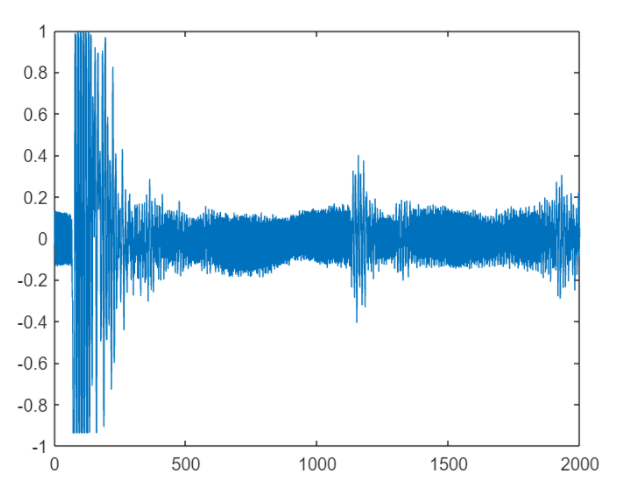
\includegraphics[width=0.5\linewidth]{figures/prefiltered.PNG}
    \caption{Pre-filtered average subtracted only}
\end{figure}
 
The low-pass filter was a 30-order Tukey window filter
with an alpha of 0.5 and a cutoff frequency of 22.16kHz. Its stopband lobes are aligned such that the 25kHz
"jamming" falls directly into one of the cracks. The high-pass filter, meanwhile, is a 61-order least-squares
 filter with a cutoff which targets only the DC component. Using two cascaded filters resulted in a lower total
 order than a single bandpass filter.

\begin{figure}[H]
    \centering
    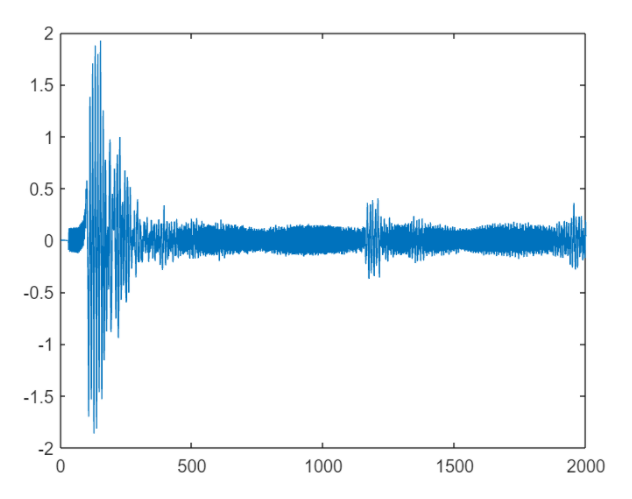
\includegraphics[width=0.5\linewidth]{figures/debiased.PNG}
    \caption{High-pass filtered, DC bias removed}
\end{figure}

An infinite impulse response (IIR) filter, specifically an elliptic filter, would allow for a much lower-order
 filter which would be faster to run, but the need to preserve phase relations meant we restricted ourselves to
 finite impulse response filters to be on the safe side, as FIR filters ensure a linear phase response. Elliptic
 IIR filters do not distort phase too badly, but enough that some amount of distortion is visible in the final
 display.

\begin{figure}[H]
    \centering
    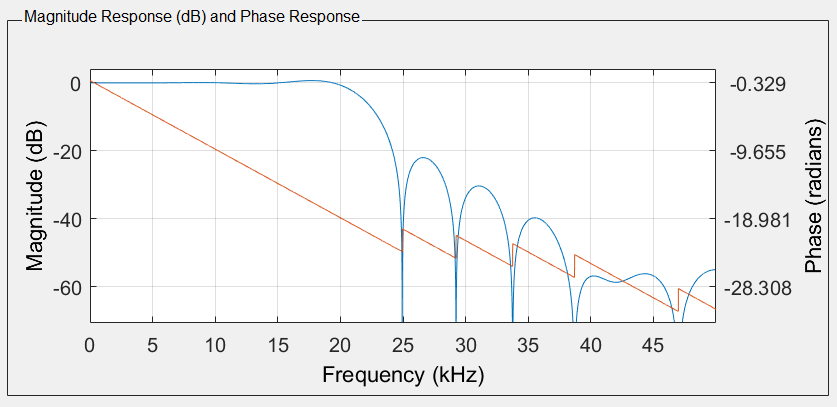
\includegraphics[width=0.5\linewidth]{figures/tukey.PNG}
    \caption{Pre-filtered average subtracted only}
\end{figure}

\begin{figure}[H]
    \centering
    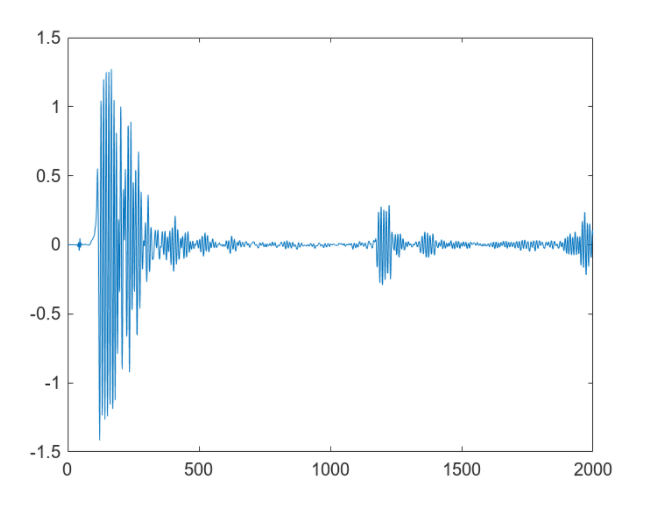
\includegraphics[width=0.5\linewidth]{figures/denoised.PNG}
    \caption{Low-pass filtered, high frequencies removed}
\end{figure}

We decided to place this block first, as the noise-reduced signal is much simpler to deal with when implementing
 the calibration stage than the raw data signal. 
\newpage
% !TEX root =./main.tex

\section{Block 2: Calibration}

The calibration block detects the sonar transmissions, shifts the data in the time domain so that the start
 of the arrays line up with the transmit time, zeros out the transmission, and normalizes the received signal
 across the arrays. To determine where the transmission occurs, the block looks for 10 consecutive samples where
 the absolute value of the signal exceeds 0.08. Then, to determine where it ends, it waits for 30 consective
 samples with a level below 0.04. From there, it shifts the data left to align the array start with the
 transmission's start. To normalize the signal magnitudes, the block examines four signals to find the maximum
 absolute values in each and applies the necessary gain to bring each signal up to the same strength as The
 strongest signal.

To optimize for speed, the calibration stage was made into a unified module instead of a distinct stage 1a and
 stage 1b. By using the already-filtered signal, a much simpler (and therefore faster and less error-prone)
 approach was feasible.  
\newpage
% !TEX root =./main.tex
\section{Block 3 : Time Gain Compensation - Nick Csicsila}

As sound travels, it attenuates through geometric spreading.  As a result, the magnitude of the second reflected pulse is significantly lower. Therefore, the program must compensate to increase the magnitudes of the two pulses back to the original magnitude of 1. 
    The samples must first be converted into distance. This is easily accomplished using the following conversion.
    \begin{align*}
     \frac{\text{Sample Index}}{F_s} \cdot c_{\text{sound}}    
    \end{align*}
    

    Although the speaker has some degree of directivity, the best results were found using the inverse- square law $(I \propto  \frac{1} {r^2} )$. 

    \begin{figure}[H]
        \centering
        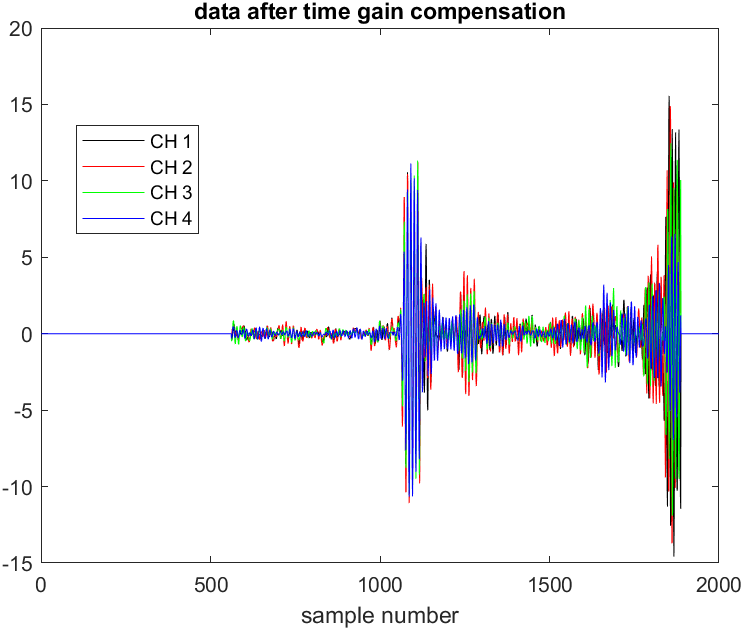
\includegraphics[width=0.5\linewidth]{figures/time_gain_1.png}
        \caption{Data after time gain compensation}
        \label{fig:time_gain1}
    \end{figure}

    \ref{fig:time_gain1}

 
\newpage
% !TEX root =./main.tex

\section{Block 4}
 
\newpage
% !TEX root =./main.tex

\section{Block 5: Beamforming - Victor Chen}

Beamforming is a signal processing technique used to spatially direct signals, enhancing desired signals while suppressing other signals with interference. A delay-and-sum beamforming algorithm is applied to the four-channel system of uniformly spaced linear sensor array of four omnidirectional microphones. Assuming the signal source is in the far field, the incoming wave fronts are approximately linear, enabling the computation of beam angle for each integer sample delay k.

The goal for the beamforming block is to use the delay-and-sum beamforming function 
\begin{align*}
    Beams[k,n] = X_1[n]+X_2[n+k]+X_3[n+2*k]+X+4[n+3*k]
\end{align*}
to spatially focus and enhance signals from a specific direction across our four-channel system.


\subsection{Implementation}

This block is designed to perform beamforming across 4,000 samples from the four channels. Given the need for multiple iterations, it is crucial to balance between processing speed and output quality.

To optimize the beamforming function, we utilize \textsc{MATLAB}'s linear vectorization and precomputing capabilities, enabling faster and more efficient processing by operating on entire data arrays simultaneously instead of relying solely on iterative loops.

\begin{figure}[H]
    \centering
    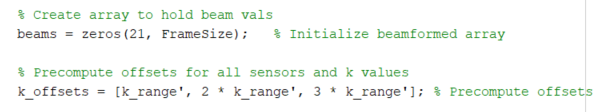
\includegraphics[width=0.5\linewidth]{figures/beamform_fig1.png}
    \caption{Precomuting Equations}
    \label{fig:precomputing_equations}
\end{figure}

The first optimization method involves precomputing the array to store the beams and the offsets for all sensors. This approach preloads the necessary matrices, eliminating the need for dynamic resizing or appending during runtime, which can significantly slow down the program. As illustrated in Figure 1, the k\_offsets for the delays are computed in a single step using vectorized operations. Additionally, a beams array is preallocated in advance to hold the calculated beams, ensuring optimal memory usage and faster processing.

\begin{figure}[H]
    \centering
    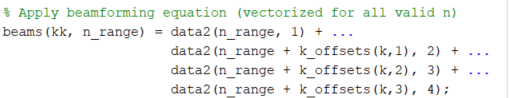
\includegraphics[width=0.5\linewidth]{figures/beamform_fig2.png}
    \caption{Beamforming Computation}
    \label{fig:beamforming_computation}
\end{figure}

The second optimization method involves performing beamforming calculations across all 4,000 samples simultaneously, rather than iterating through each index individually. This reduces the number of loops, making the process much more efficient.



\subsection{Analysis}

After developing the beamforming function, test data was generated to evaluate its performance. The test data consisted of four channels of in-phase sine waves, defined by the equation \textit{sample} = sin(\textit{t}/40), where \textit{t} ranged from 1 to 4,000. After ensuring the function works with the test data, I used data2 directly from the project.

\begin{figure}[H]
    \centering
    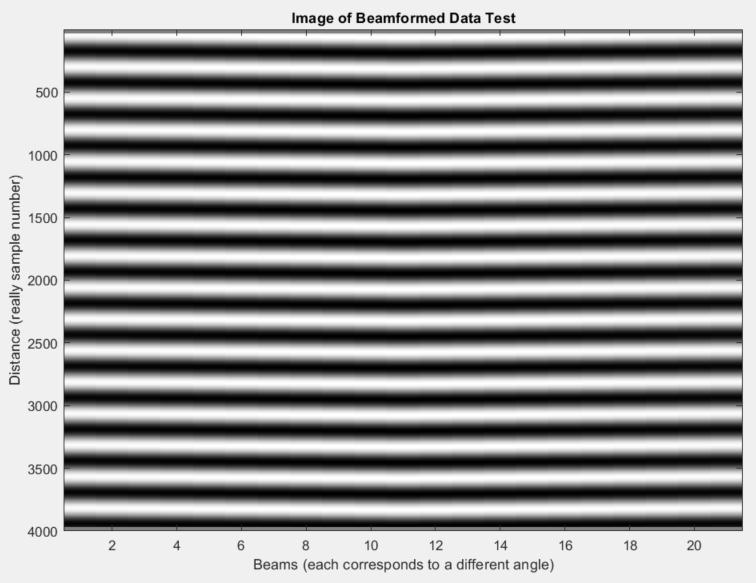
\includegraphics[width=0.5\linewidth]{figures/beamform_fig3.png}
    \caption{Output for Testing with sin(t/40) wave}
    \label{fig:sinwave_output}
\end{figure}

As shown in Figure 3, each black-and-white horizontal line represents a wave. With 4,000 samples in the equation sin(\textit{t}/40), this corresponds to approximately 16 waves. The figure confirms this, demonstrating that the beamforming function performs as expected. It is important to note that the waves are evenly horizontal due to the in-phase channels, however, as the frequency of the waves increases, the evenness of the waves will begin to separate.

\begin{figure}[H]
    \centering
    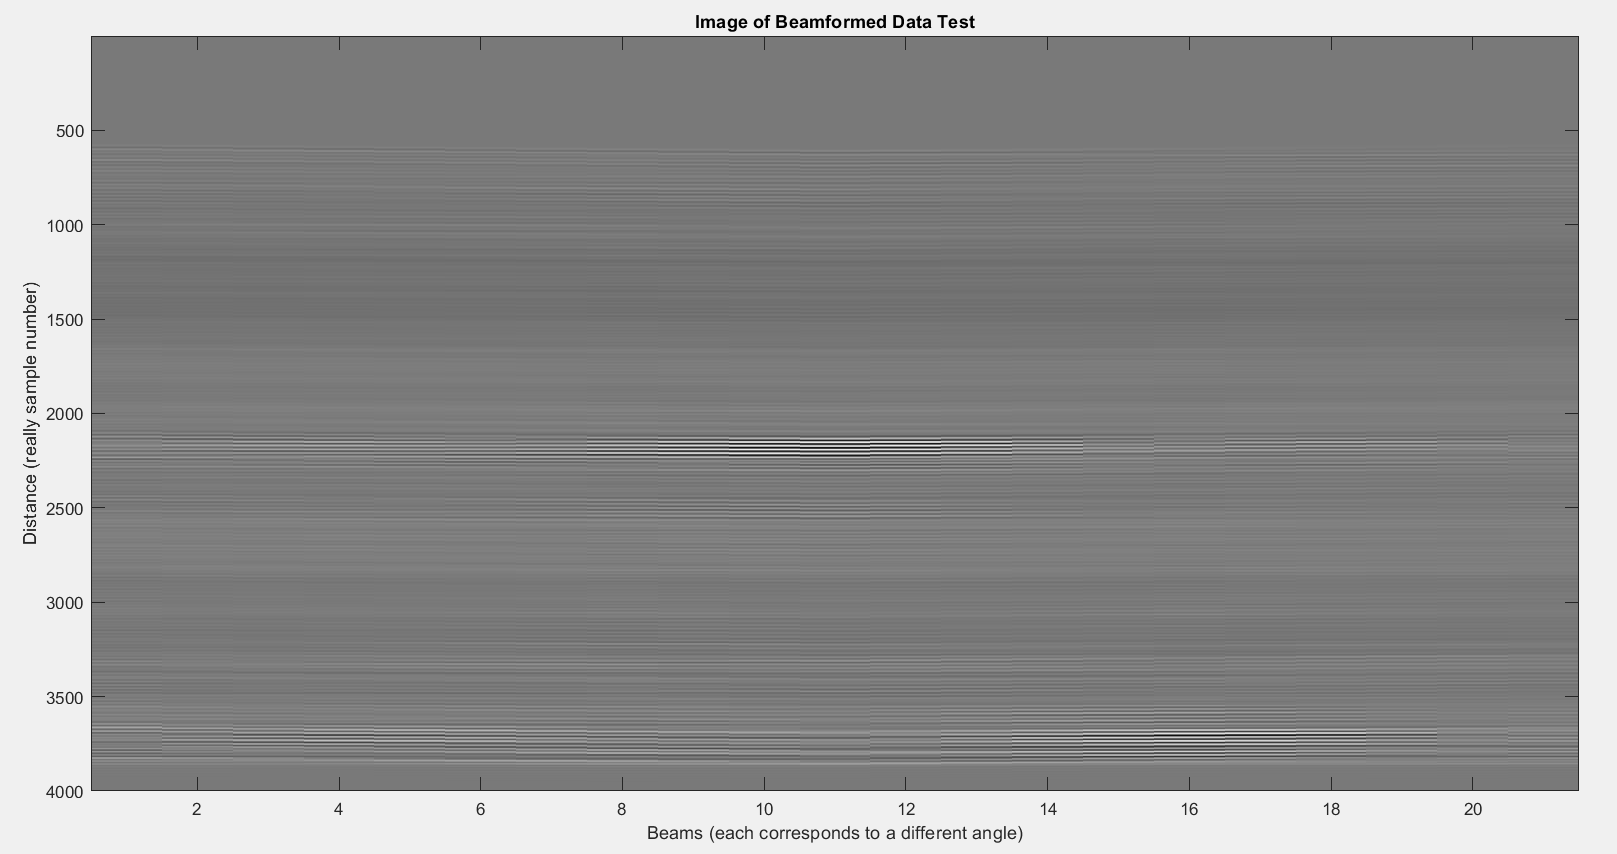
\includegraphics[width=0.5\linewidth]{figures/beamform_fig4.png}
    \caption{Beamform Output from Data}
    \label{fig:final_beamform_output}
\end{figure}

As shown in Figure 4, the beamform output of data2 reveals two regions where the signal strength is highest. These are represented by two prominent white "blobs"--one near the center and another near the bottom-right corner of the beamformed image. These regions indicate areas where the waves return well-constructed, suggesting the presence of an object that the waves interacted with.

\begin{figure}[H]
    \centering
    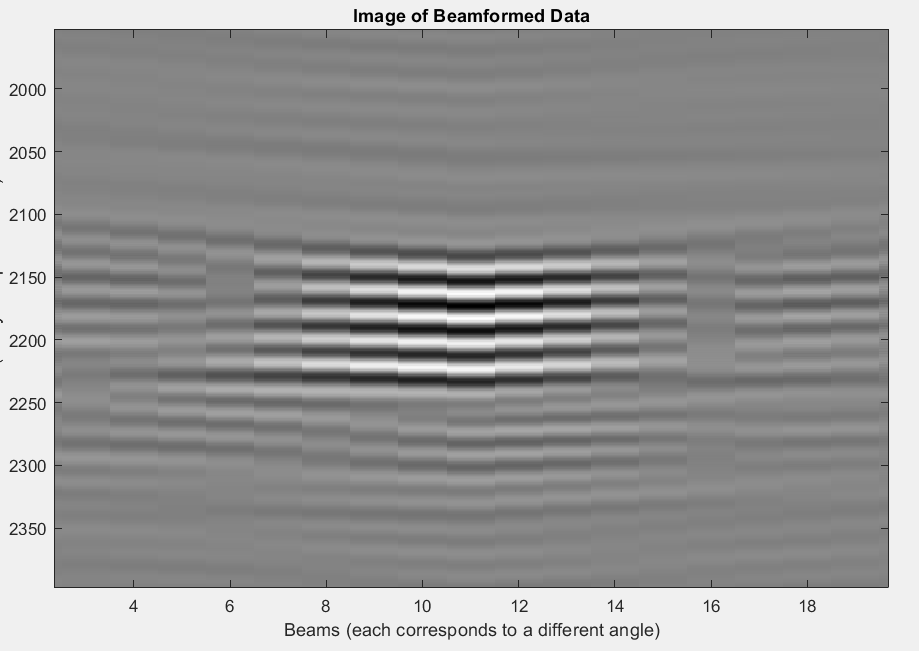
\includegraphics[width=0.5\linewidth]{figures/beamform_fig5.png}
    \caption{Zoomed In Beamform Output}
    \label{fig:zoomed_in_beamform_output}
\end{figure}

By zooming into the center of the beamform image in Figure 5, we can see that while the signal strength is high, each beam is still slightly offset. This offset may be due to inaccuracies in my delay calculations or it might be due to the geometry/spacing of the sensors. Plenty of time was spent on trying to correct the offset by shifting beams, however none were successful. More work will need to be done to correct this issue.


The beamforming function achieved an average execution time of 0.0023155 seconds, a substantial improvement compared to pre-optimization runs, which took tens of seconds. This demonstrates a significant increase in computational efficiency for beamforming.
  
\newpage
\input{./06-conclusion} 


\end{document}
